\chapter{Solutions of chapter 1 \\
	Basic formal concepts}\label{chap1}
\section{Solutions Exercises}\label{sec11}
\begin{enumerate}[leftmargin=*]
\item \textit{The court case: the blue or green cap}
	
A cab was involved in a hit and run accident at night. There are two cab companies in the town: blue and green. The former has 150 cabs, and the latter 850 cabs. A witness said that a blue cab was involved in the accident; the court tested his/her reliability under the same circumstances, and got that 80\% of the times the witness correctly identified the color of the cab. \textit{what is the probability that the color of the cab involved in the accident was blue given that the witness said it was blue?}
	
\textbf{Answer}
	
Set $WB$ and $WG$ equal to the events that the witness said the cab was blue and green, respectively. Set $B$ and $G$ equal to the events that the cabs are blue and green, respectively. We need to calculate $P(B|WB)$, then:
	
\begin{align}
	P(B|WB)&=\frac{P(B,WB)}{P(WB)}\\
	&=\frac{P(WB|B)\times P(B)}{P(WB|B)\times P(B)+(1-P(WB|B))\times (1-P(B))}\nonumber\\
	&=\frac{0.8\times 0.15}{0.8\times 0.15+0.2\times 0.85}\nonumber\\
	&=0.41\nonumber
\end{align}
	
	
\item \textit{The Monty Hall problem}
	
What is the probability of winning a car in the \textit{Monty Hall problem} switching the decision if there are four doors, where there are three goats and one car? Solve this problem analytically and computationally.  What if there are $n$ doors, $n-1$ goats and one car?
	
\textbf{Answer}
	
Let's name $P_i$ the event \textit{contestant picks door No. $i$}, $H_i$ the event \textit{host picks door No. $i$}, and $C_i$ the event \textit{car is behind door No. $i$}. Let's assume that the contestant picked door number 1, and the host picked door number 3, then the contestant is interested in the probability of the event $P(C_i|H_3,P_1), i = 2 \ \text{or} \ 4$. Then, $P(H_3|C_3,P_1)=0$, $P(H_3|C_2,P_1)=P(H_3|C_4,P_1)=1/2$ and $P(H_3|C_1,P_1)=1/3$. Then,  
	
\begin{align}
	P(C_i|H_3,P_1)&= \frac{P(C_i,H_3,P_1)}{P(H_3,P_1)}\\
	&= \frac{P(H_3|C_i,P_1)P(C_i|P_1)P(P_1)}{P(H_3|P_1)\times P(P_1)}\nonumber\\
	&= \frac{P(H_3|C_i,P_1)P(C_i)}{P(H_3|P_1)}\nonumber\\
	&=\frac{1/2\times 1/4}{1/3}\nonumber\\
	&=\frac{3}{8},\nonumber
\end{align}
where the third equation uses the fact that $C_i$ and $P_i$ are independent events, and $P(H_3|P_1)=1/3$ due to this depending just on $P_1$ (not on $C_i$).
	
Therefore, changing the initial decision increases the probability of getting the car from 1/4 to 3/8!
	
Let's check the case with $n$ doors, and assume that the contestant picks the door No. $1$, the car is behind the door No. $n$, and the host, who knows what is behind each door, opens any of the remaining $n-2$ doors, where there is a goat. The contestant is interested in the probability of the event:
{\tiny{
\begin{align}
	P\left( C_{n} | (H_2 \cup  \ldots \cup H_{n-1}) \cap P_1 \right)  & = 
	\frac{P\left( (H_2 \cup H_3 \cup \ldots \cup H_{n-1}) | C_{n} \cap P_1\right) P(C_{n} | P_1) P(P_1)}{P\left( (H_2 \cup H_3 \cup \ldots \cup H_{n-1}) | P_1 \right) P(P_1)} \\
	& = \frac{\left[ P\left( H_2 | C_{n} \cap P_1\right) + \ldots P\left( H_{n-1}| C_{n} \cap P_1\right) \right] P(C_{n})}{P\left( H_2 | P_1 \right) + P\left( H_3 | P_1 \right) + \ldots + P\left( H_{n-1} | P_1 \right)} \nonumber\\
	& = \frac{1 \times \left( \frac{1}{n} \right) }{\frac{1}{n-1} + \frac{1}{n-1} + \ldots + \frac{1}{n-1}} \nonumber\\
	& = \left( \frac{1}{n}\right) \left( \frac{n-1}{n-2}\right).\nonumber 
\end{align}
}}	
In general, the probability of winning the car changing the pick is $\frac{1}{n} \frac{n-1}{n-2}$, while the probability of winning given no change is $\frac{1}{n}$. Given that $\frac{1}{n} \frac{n-1}{n-2} > \frac{1}{n}$ for all $n \geq 3$, where the difference between both probabilities is  $\frac{1}{n(n-2)}$. We observe that as the number of doors increases, the difference between the two probabilities becomes zero.
	
Let's see a code for the general setting,

\begin{tcolorbox}[enhanced,width=4.67in,center upper,
	fontupper=\large\bfseries,drop shadow southwest,sharp corners]
\textit{R code. The Monty Hall Problem}
\begin{VF}
\begin{lstlisting}[basicstyle=\footnotesize, language=R]
set.seed(0101) # Set simulation seed
S <- 100000 # Simulations
Game <- function(opt = 3){
# opt: number of options. opt > 2
opts <- 1:opt 
car <- sample(opts, 1) # car location
guess1 <- sample(opts, 1) # Initial guess
		
if(opt == 3 && car != guess1) {
 host <- opts[-c(car, guess1)]
 } else {
 host <- sample(opts[-c(car, guess1)], 1)
}
			
win1 <- guess1 == car # Win given no change
			
if(opt == 3) {
 guess2 <- opts[-c(host, guess1)]
 } else {
 guess2 <- sample(opts[-c(host, guess1)], 1)
 } 
			
win2 <- guess2 == car # Win given change
			
return(c(win1, win2))
}
#Win probabilities
Prob <- rowMeans(replicate(S, Game(opt = 4))) 
#Winning probabilities no changing door
Prob[1]
0.25151
#Winning probabilities changing door
Prob[2]
0.37267
\end{lstlisting}
\end{VF}
\end{tcolorbox}

\item Solve the health insurance example using a Gamma prior in the rate parametrization, that is, $\pi(\lambda)=\frac{\beta_0^{\alpha_0}}{\Gamma(\alpha_0)}\lambda^{\alpha_0-1}\exp\left\{-\lambda\beta_0\right\}$.

\textbf{Answer}

First, we get the posterior distribution,
\begin{align}
	\pi\left(\lambda | \textbf{y}  \right) & = \left( \frac{\beta_0^{\alpha_0}}{\Gamma(\alpha_0)} \lambda^{\alpha_0 - 1} e^{-\lambda \beta_0} \right) \left(  \prod_{i = 1}^{N} \frac{\lambda^{y_i} e^{-\lambda}}{y_i!} \right)
\end{align}

\begin{align}
	& = \left( \frac{\beta_0^{\alpha_0}}{\Gamma(\alpha_0)} \lambda^{\alpha_0 - 1} e^{-\lambda \beta_0} \right) \left( \frac{\lambda^{\sum_{i = 1}^{N} y_i} e^{-N \lambda}}{\prod_{i = 1}^{N} y_i !}\right) \nonumber\\ 
	& = \left(  \frac{\beta_0^{\alpha_0}}{\Gamma(\alpha_0)} \frac{1}{\prod_{i = 1}^{N} y_i !} \right) \lambda^{\sum_{i = 1}^{N} y_i + \alpha_0 - 1} e^{-\lambda\left( \beta_0 + N \right) } \nonumber \\
	& \propto \lambda^{\sum_{i = 1}^{N} y_i + \alpha_0 - 1} e^{-\lambda\left( \beta_0 + N \right) }.\\ \nonumber 
\end{align}

The last expression is the kernel of a Gamma distribution with parameters $\alpha_n = \sum_{i = 1}^{N} y_i + \alpha_0$ and $\beta_n = \beta_0 + N$.

Given that $\int_{0}^{\infty} \pi\left( \lambda | \textbf{y} \right) d\lambda = 1 $, then the constant of proportionality in the last expression is $\Gamma\left( \alpha_n\right) / \beta_n^{\alpha_n}$. Therefore the posterior density function $\pi\left(\lambda | \textbf{y}  \right)$ is $ G\left(\alpha_n, \beta_n \right)$.

The posterior mean is

\begin{align}
	E\left[ \lambda | \textbf{y}\right] & = \frac{\alpha_n}{\beta_n}  \\ 
	& = \frac{\sum_{i = 1}^{N} y_i + \alpha_0}{\beta_0 + N} \nonumber \\ 
	& = \left( \frac{N}{\beta_0 + N}\right) \bar{y} + \left( \frac{\beta_0}{\beta_0 + N}\right) \frac{\alpha_0}{\beta_0}  \nonumber \\
	& = w \bar{y} + \left( 1 - w \right) E\left[ \lambda \right], \nonumber 
\end{align}

where $w = \frac{N}{\beta_0 + N}$, $\bar{y}$ is the sample mean, and $E\left[ \lambda \right]  = \frac{\alpha_0}{\beta_0}$.

The posterior predictive distribution is given by

\begin{align}
	\pi\left(Y_0 | \textbf{y} \right) & = \int_{0}^{\infty} \frac{\lambda^{y_0} e^{-\lambda}}{y_0!} \pi\left(\lambda | \textbf{y}  \right) d \lambda\\
    & = \int_{0}^{\infty} \left( \frac{\lambda^{y_0} e^{-\lambda}}{y_0!} \right) \left( \frac{\beta_n^{\alpha_n}}{\Gamma(\alpha_n)} \lambda^{\alpha_n - 1} e^{-\lambda \beta_n} \right) d\lambda \nonumber \\
	& = \frac{\beta_n^{\alpha_n}}{\Gamma\left( \alpha_n\right) y_0 !} \int_{0}^{\infty} \lambda^{y_0 + \alpha_n - 1} e^{-\lambda \left( 1 + \beta_n\right)} d\lambda \nonumber \\
	& = \frac{\beta_n^{\alpha_n}}{\Gamma\left( \alpha_n\right) y_0 !} \frac{\Gamma\left( y_0 + \alpha_n \right) }{\left( 1 + \beta_n \right)^{y_0 + \alpha_n}} \nonumber\\
	& = \frac{\Gamma\left( y_0 + \alpha_n \right)}{\Gamma\left( \alpha_n \right) y_0 !} \left( \frac{1}{1 + \beta_n}\right)^{y_0} \left(\frac{\beta_n}{1 + \beta_n} \right)^{\alpha_n} \nonumber
\end{align}

\begin{align}
	& = \frac{\left( y_0 + \alpha_n - 1\right)!}{\left( \alpha_n - 1\right)! y_0 ! } \left( \frac{1}{1 + \beta_n}\right)^{y_0} \left(\frac{\beta_n}{1 + \beta_n} \right)^{\alpha_n} \nonumber \\	
	& = \binom{y_0 + \alpha_n - 1}{y_0} \left( \frac{1}{1 + \beta_n}\right)^{y_0} \left(\frac{\beta_n}{1 + \beta_n} \right)^{\alpha_n}. \nonumber 
\end{align}

Therefore $Y_0 | y \sim NB(\alpha_n, p_n) $ where $p_n = \frac{1}{1 + \beta_n}$.

To use empirical Bayes, we have the following setting

\begin{equation*}
	\left[ \hat{\alpha_0} \hat{\beta_0}\right] = \arg \max_{\alpha_0, \beta_0} \ln (p(\textbf{y})), 
\end{equation*}
where
\begin{align}
	p(y) & = \int_{0}^{\infty} \left( \frac{\beta_0^{\alpha_0}}{\Gamma(\alpha_0)} \lambda^{\alpha_0 - 1} e^{-\lambda \beta_0} \right) \left(  \prod_{i = 1}^{N} \frac{\lambda^{y_0} e^{-\lambda}}{y_0!} \right)  d\lambda \\
	& = \left(  \frac{\beta_0^{\alpha_0}}{\Gamma(\alpha_0) \prod_{i = 1}^{N} y_i !} \right) \int_{0}^{\infty}\lambda^{\sum_{i = 1}^{N} y_i + \alpha_0 - 1} e^{-\lambda\left( \beta_0 + N \right)} d\lambda \nonumber \\
	& = \left(  \frac{\beta_0^{\alpha_0}}{\Gamma(\alpha_0) \prod_{i = 1}^{N} y_i !} \right) \left(   \frac{\Gamma\left( \sum_{i=1}^{N} y_i + \alpha_0 \right) }{\left(\beta_0 + N\right)^{\sum_{i=1}^{N} y_i + \alpha_0} } 	\right) \nonumber \\
	& = \frac{\Gamma\left( \sum_{i=1}^{N} y_i + \alpha_0 \right)}{\Gamma(\alpha_0) \prod_{i = 1}^{N} y_i !} \left( \frac{1}{\beta_0 + N}\right)^{\sum_{i=1}^{N} y_i} \left(\frac{\beta_0}{\beta_0 + N} \right)^{\alpha_0}.\nonumber   
\end{align}

\begin{tcolorbox}[enhanced,width=4.67in,center upper,
	fontupper=\large\bfseries,drop shadow southwest,sharp corners]
	\textit{R code. Health insurance, predictive distribution using vague hyperparameters}
\begin{VF}
\begin{lstlisting}[basicstyle=\footnotesize, language=R]
set.seed(010101)
y <- c(0, 3, 2, 1, 0) # Data
N <- length(y)

# Predictive distribution
ProbBo <- function(y, a0, b0){
	N <- length(y) 
	#sample size
	aN <- a0 + sum(y) 
	# Posterior shape parameter
	bN <- b0 + N 
	# Posterior scale parameter
	p <- 1 / (bN + 1) 
	# Probability negative binomial density
	Pr <- 1 - pnbinom(0, size = aN, prob = (1 - p)) 
	# Probability of visiting the Doctor
	# Observe that in R there is a slightly 
	# different parametrization.
	return(Pr)
} 

# Using a vague prior:
a0 <- 0.001 # Prior shape parameter
b0 <- 0.001 # Prior scale parameter
PriMeanV <- a0 / b0 # Prior mean
PriVarV <- a0 / b0^2 # Prior variance
Pp <- ProbBo(y, a0 = 0.001, b0 = 0.001) 
# This setting is vague prior information.
Pp
0.67
\end{lstlisting}
\end{VF}
\end{tcolorbox}


\begin{tcolorbox}[enhanced,width=4.67in,center upper,
	fontupper=\large\bfseries,drop shadow southwest,sharp corners]
	\textit{R code. Health insurance, predictive distribution using empirical Bayes}
\begin{VF}
\begin{lstlisting}[basicstyle=\footnotesize, language=R]
	
# Using Emprirical Bayes
LogMgLik <- function(theta, y){
	N <- length(y) 
	#sample size
	a0 <- theta[1] 
	# prior shape hyperparameter
	b0 <- theta[2] 
	# prior scale hyperparameter
	aN <- sum(y) + a0 
	# posterior shape parameter
	if(a0 <= 0 || b0 <= 0){ 
		#Avoiding negative values
		lnp <- -Inf
	}else{lnp <- lgamma(aN) - sum(y)*log(b0+N) + 
	a0*log(b0/(b0+N)) - lgamma(a0)} 
    # log marginal likelihood
	return(-lnp)
}

theta0 <- c(0.01, 0.01) 
# Initial values
control <- list(maxit = 1000) 
# Number of iterations in optimization
EmpBay <- optim(theta0, LogMgLik, method = "BFGS", 
control = control, hessian = TRUE, y = y) 
# Optimization
EmpBay$convergence 
# Checking convergence
EmpBay$value # Maximum
a0EB <- EmpBay$par[1] 
# Prior shape using empirical Bayes
a0EB
128.383
b0EB <- EmpBay$par[2] 
# Prior scale using empirical Bayes
b0EB 
106.801

PriMeanEB <- a0EB / b0EB 
# Prior mean
PriVarEB <- a0EB / b0EB^2 
# Prior variance
PpEB <- ProbBo(y, a0 = a0EB, b0 = b0EB) 
# This setting is using emprical Bayes.
PpEB
0.69
\end{lstlisting}
\end{VF}
\end{tcolorbox}

\item Suppose that you are analyzing to buy a car insurance next year. To make a better decision you want to know \textit{what is the probability that you have a car claim next year?} You have the records of your car claims in the last 15 years, $\mathbf{y}=\left\{0, 1, 0, 1, 0, 1, 1, 0, 0, 1, 0, 0, 1, 1, 0\right\}$.
	
Assume that this is a random sample from a data generating process (statistical model) that is Bernoulli, $Y_i\sim Ber(p)$, and your probabilistic prior beliefs about $p$ are well described by a beta distribution with parameters $\alpha_0$ and $\beta_0$, $p\sim B(\alpha_0, \beta_0)$, then, you are interested in calculating the probability of a claim the next year $P(Y_0 = 1|\mathbf{y})$.
	
Solve this using an empirical Bayes approach and a non-informative approach where $\alpha_0=\beta_0=1$ (uniform distribution).

\textbf{Answer}

The posterior distribution is given by
	\begin{align}
		\pi\left( p | \textbf{y}\right) & = \left[ \frac{\Gamma\left( \alpha_0 + \beta_0\right) }{\Gamma\left( \alpha_0\right) \Gamma\left( \beta_0\right) } p^{\alpha_0 - 1} \left( 1 - p \right)^{\beta_0 - 1} \right] \left[ \prod_{i = 1}^{N} p^{y_i} \left( 1 - p\right)^{1 - y_i} \right]  \\
		& = \frac{\Gamma\left( \alpha_0 + \beta_0\right) }{\Gamma\left( \alpha_0\right) \Gamma\left( \beta_0\right) } p^{\sum_{i = 1}^{N} y_i + \alpha_0 - 1} \left( 1 - p\right)^{\beta_0 + N - \sum_{i = 1}^{N} y_i - 1} \nonumber \\
		& \propto  p^{\sum_{i = 1}^{N} y_i + \alpha_0 - 1} \left( 1 - p\right)^{\beta_0 + N - \sum_{i = 1}^{N} y_i - 1}. \nonumber
	\end{align}
	
	The last expression is the kernel of a Beta distribution with parameters $\alpha_n = \sum_{i = 1}^{N} y_i + \alpha_0$ and $\beta_n = \beta_0 + N - \sum_{i = 1}^{N} y_i$. Thus, the posterior mean is 
	
	\begin{align}
		E\left[ p | \textbf{y}\right] & = \frac{\alpha_n}{\alpha_n + \beta_n} \nonumber \\
		& = \frac{\sum_{i = 1}^{N} y_i + \alpha_0}{\alpha_0 + \beta_0 + N} \\
		& = \frac{N \bar{y}}{\alpha_0 + \beta_0 + N} + \frac{\alpha_0}{\alpha_0 + \beta_0 + N} \nonumber \\
		& = \frac{N}{\alpha_0 + \beta_0 + N} \left( \bar{y} \right) + \frac{\alpha_0 + \beta_0}{\alpha_0 + \beta_0 + N} \left( \frac{\alpha_0}{\alpha_0 + \beta_0}\right) \nonumber \\
		& = w \left( \bar{y}\right) + (1 - w) E\left[ p \right], \nonumber  
	\end{align}
	
	where $w = \frac{N}{\alpha_0 + \beta_0 + N}$, $\bar{y}$ is the sample mean, and $E\left[ p \right]  = \frac{\alpha_0}{\alpha_0 + \beta_0}$ is the prior mean.
	
	The posterior predictive distribution of claim the next year is given by
	
	\begin{align}
		\pi(Y_0 = 1| \textbf{y}) & = \int_{0}^{1}  P(Y_0 = 1| \textbf{y}, p) \pi\left( p | \textbf{y}\right) dp \nonumber \\
		& = \int_{0}^{1}  p  \times \pi\left( p | \textbf{y}\right) dp \nonumber \\
		& =  \mathbb{E}\left[ p | \textbf{y} \right]   \nonumber \\
		& =  \frac{\alpha_n}{\alpha_n + \beta_n}.
	\end{align}
	
	To use empirical Bayes, we have the following setting
	
	\begin{equation*}
		\left[ \hat{\alpha_0} \hat{\beta_0}\right] = \arg \max_{\alpha_0, \beta_0} \ln (p(\textbf{y})), 
	\end{equation*}

where
	
	\begin{align}
		p(\textbf{y}) & = \int_{0}^{1} \left[ \frac{\Gamma\left( \alpha_0 + \beta_0\right) }{\Gamma\left( \alpha_0\right) \Gamma\left( \beta_0\right) } p^{\alpha_0 - 1} \left( 1 - p\right)^{\beta_0 - 1} \right]  \left[ \prod_{i = 1}^{N}  \left( 1 - p\right)^{1 - y_i}  \right] dp \\
		& =  \frac{\Gamma\left( \alpha_0 + \beta_0\right) }{\Gamma\left( \alpha_0\right) \Gamma\left( \beta_0\right) }  \int_{0}^{1} p^{\sum_{i = 1}^{N} y_i + \alpha_0 - 1} \left( 1 - p \right)^{\beta_0 + N - \sum_{i = 1}^{N} y_i -1} dp \nonumber \\
		& =  \frac{\Gamma\left( \alpha_0 + \beta_0\right) }{\Gamma\left( \alpha_0\right) \Gamma\left( \beta_0\right)} \frac{\Gamma\left(\sum_{i = 1}^{N} y_i + \alpha_0 \right) \Gamma\left(\beta_0 + N - \sum_{i = 1}^{N} y_i \right) }{\Gamma\left( \alpha_0 + \beta_0 + N\right) }.\nonumber 
	\end{align}

\begin{tcolorbox}[enhanced,width=4.67in,center upper,
	fontupper=\large\bfseries,drop shadow southwest,sharp corners]
	\textit{R code. Car claim, predictive distribution using vague hyperparameters}
\begin{VF}
\begin{lstlisting}[basicstyle=\footnotesize, language=R]
set.seed(010101)
y <- c(0, 1, 0, 1, 0, 1, 1, 0, 0, 1, 0, 0, 1, 1, 0) 
# Data
N <- length(y)

#require(TailRank)

# Predictive distribution
ProbBo <- function(y, a0, b0){
	N <- length(y) 
	#sample size
	aN <- a0 + sum(y) 
	# Posterior shape parameter
	bN <- b0 + N - sum(y) 
	# Posterior scale parameter
	pr <- aN / (aN + bN) 
	# Probability of a claim the next year
	return(pr)
} 

# Using a vague prior:
a0 <- 1 # Prior shape parameter
b0 <- 1 # Prior scale parameter
PriMeanV <- a0 / (a0 + b0) 
# Prior mean
PriVarV <- (a0*b0) / (((a0+b0)^2)*(a0+b0+1)) 
# Prior variance

Pp <- ProbBo(y, a0 = 1, b0 = 1)
# This setting is defining vague prior information.
# The probability of a claim 
0.47

\end{lstlisting}
\end{VF}
\end{tcolorbox}


\begin{tcolorbox}[enhanced,width=4.67in,center upper,
	fontupper=\large\bfseries,drop shadow southwest,sharp corners]
	\textit{R code. Car claim, predictive distribution using empirical Bayes}
\begin{VF}
\begin{lstlisting}[basicstyle=\footnotesize, language=R]
# Using Emprirical Bayes
LogMgLik <- function(theta, y){
	N <- length(y) 
	#sample size
	a0 <- theta[1] 
	# prior shape hyperparameter
	b0 <- theta[2] 
	# prior scale hyperparameter
	aN <- sum(y) + a0 
	# posterior shape parameter
	if(a0 <= 0 || b0 <= 0){ 
		#Avoiding negative values
		lnp <- -Inf
	}else{lnp <- lgamma(a0+b0) + lgamma(aN) + 
	lgamma(b0+N-sum(y)) -lgamma(a0) -lgamma(b0) - 
	lgamma(a0+b0+N)} 
	# log marginal likelihood
	return(-lnp)
}

theta0 <- c(0.1, 0.1) 
# Initial values
control <- list(maxit = 1000) 
# Number of iterations in optimization
EmpBay <- optim(theta0, LogMgLik, method = "BFGS", 
control = control, hessian = TRUE, y = y) 
# Optimization
EmpBay$convergence 
# Checking convergence
EmpBay$value # Maximum
a0EB <- EmpBay$par[1] 
# Prior shape using empirical Bayes
b0EB <- EmpBay$par[2] 
# Prior scale using empirical Bayes

PriMeanEB <- a0EB /(a0EB + b0EB)  
# Prior mean
PriVarEB <- (a0EB*b0EB)/(((a0EB+b0EB)^2)*(a0EB+b0EB+1)) 
# Prior variance

PpEB <- ProbBo(y, a0 = a0EB, b0 = b0EB)
 # This setting is using empirical Bayes.
PpEB
0.47

\end{lstlisting}
\end{VF}
\end{tcolorbox}


\begin{tcolorbox}[enhanced,width=4.67in,center upper,
	fontupper=\large\bfseries,drop shadow southwest,sharp corners]
	\textit{R code. Car claim, density plots}
\begin{VF}
\begin{lstlisting}[basicstyle=\scriptsize, language=R]
# Density figures
lambda <- seq(0.001, 1, 0.001) 
# Values of lambda
VaguePrior <- dbeta(lambda, shape1 = a0, shape2 = b0)
EBPrior <- dbeta(lambda, shape1 = a0EB, shape2 = b0EB)
PosteriorV <- dbeta(lambda, shape1 = a0 + sum(y), 
shape2 = b0 + N - sum(y))
PosteriorEB <- dbeta(lambda, shape1 = a0EB + sum(y),
 shape2 = b0EB + N - sum(y))

# Likelihood function
Likelihood <- function(theta, y){
	LogL <- dbinom(y, 1, theta, log = TRUE)
	#  LogL <- dbern(y, theta)
	Lik <- prod(exp(LogL))
	return(Lik)
}


Liks <- sapply(lambda, function(par) {
	Likelihood(par, y = y)})
Sc <- max(PosteriorEB)/max(Liks) 
#Scale for displaying in figure
LiksScale <- Liks * Sc

data <- data.frame(cbind(lambda, VaguePrior, EBPrior, 
PosteriorV, PosteriorEB, LiksScale)) 
#Data frame

require(ggplot2) 
# Cool figures
require(latex2exp) 
# LaTeX equations in figures
require(ggpubr) 
# Multiple figures in one page

fig1 <- ggplot(data = data, aes(lambda, VaguePrior)) + 
geom_line() +  
xlab(TeX("$p$")) + ylab("Density") +
ggtitle("Prior: Vague Beta") 

fig2 <- ggplot(data = data, aes(lambda, EBPrior)) + 
geom_line() +  
xlab(TeX("$p$")) + ylab("Density") +
ggtitle("Prior: Empirical Bayes Beta")

fig3 <- ggplot(data = data, aes(lambda, PosteriorV)) + 
geom_line() +  
xlab(TeX("$p$")) + ylab("Density") +
ggtitle("Posterior: Vague Beta")

fig4 <- ggplot(data = data, aes(lambda, PosteriorEB)) + 
geom_line() +  
xlab(TeX("$p$")) + ylab("Density") +
ggtitle("Posterior: Empirical Bayes Beta")

FIG <- ggarrange(fig1, fig2, fig3, fig4,
ncol = 2, nrow = 2)

annotate_figure(FIG,
top = text_grob("Vague versus Empirical Bayes: 
Beta-Bernoulli model", color = "black", 
face = "bold", size = 14))
			
\end{lstlisting}
\end{VF}
\end{tcolorbox}

\begin{figure}[!h]
	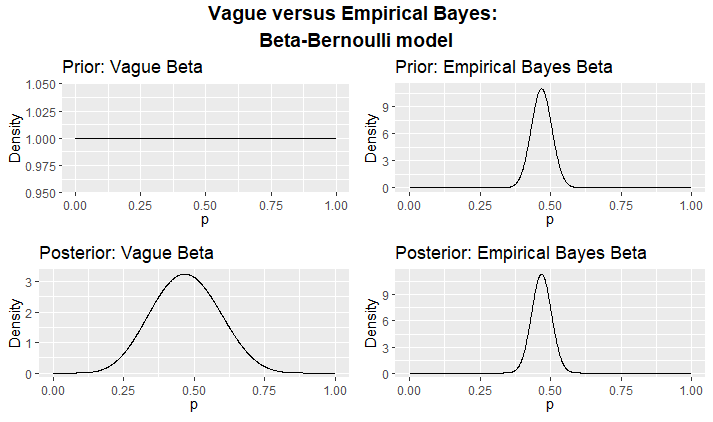
\includegraphics[width=340pt, height=200pt]{Chapters/chapter1/figures/BerBeta.png}
	%%\centerline{\epsfig{/Chapters/chapter1/figures/cat.eps,width=.8\textheight,height=.4\textwidth}}
	\caption[List of figure caption goes here]{Vague versus Empirical Bayes: Bernoulli-Beta model.}\label{fig11}
\end{figure}

\begin{tcolorbox}[enhanced,width=4.67in,center upper,
fontupper=\large\bfseries,drop shadow southwest,sharp corners]
\textit{R code. Car claim, prior, likelihood and posterior density plots}
\begin{VF}
\begin{lstlisting}[basicstyle=\scriptsize, language=R]
# Prior, likelihood and posterior: 
#Empirical Bayes Binonial-Beta model
dataNew <- data.frame(cbind(rep(lambda, 3), 
c(EBPrior, PosteriorEB, LiksScale),
rep(1:3, each = 1000))) 
#Data frame

colnames(dataNew) <- c("Lambda", "Density", "Factor")
dataNew$Factor <- factor(dataNew$Factor, levels=c("1", "3", 
"2"), labels=c("Prior", "Likelihood", "Posterior"))

ggplot(data = dataNew, aes_string(x = "Lambda", 
y = "Density", group = "Factor")) + 
geom_line(aes(color = Factor)) +
xlab(TeX("$\\lambda$")) + ylab("Density") +
ggtitle("Prior, likelihood and posterior: Empirical Bayes
 Poisson-Gamma model") +
guides(color=guide_legend(title="Information")) +
scale_color_manual(values = c("red", "yellow", "blue"))

\end{lstlisting}
\end{VF}
\end{tcolorbox}

\begin{figure}[!h]
	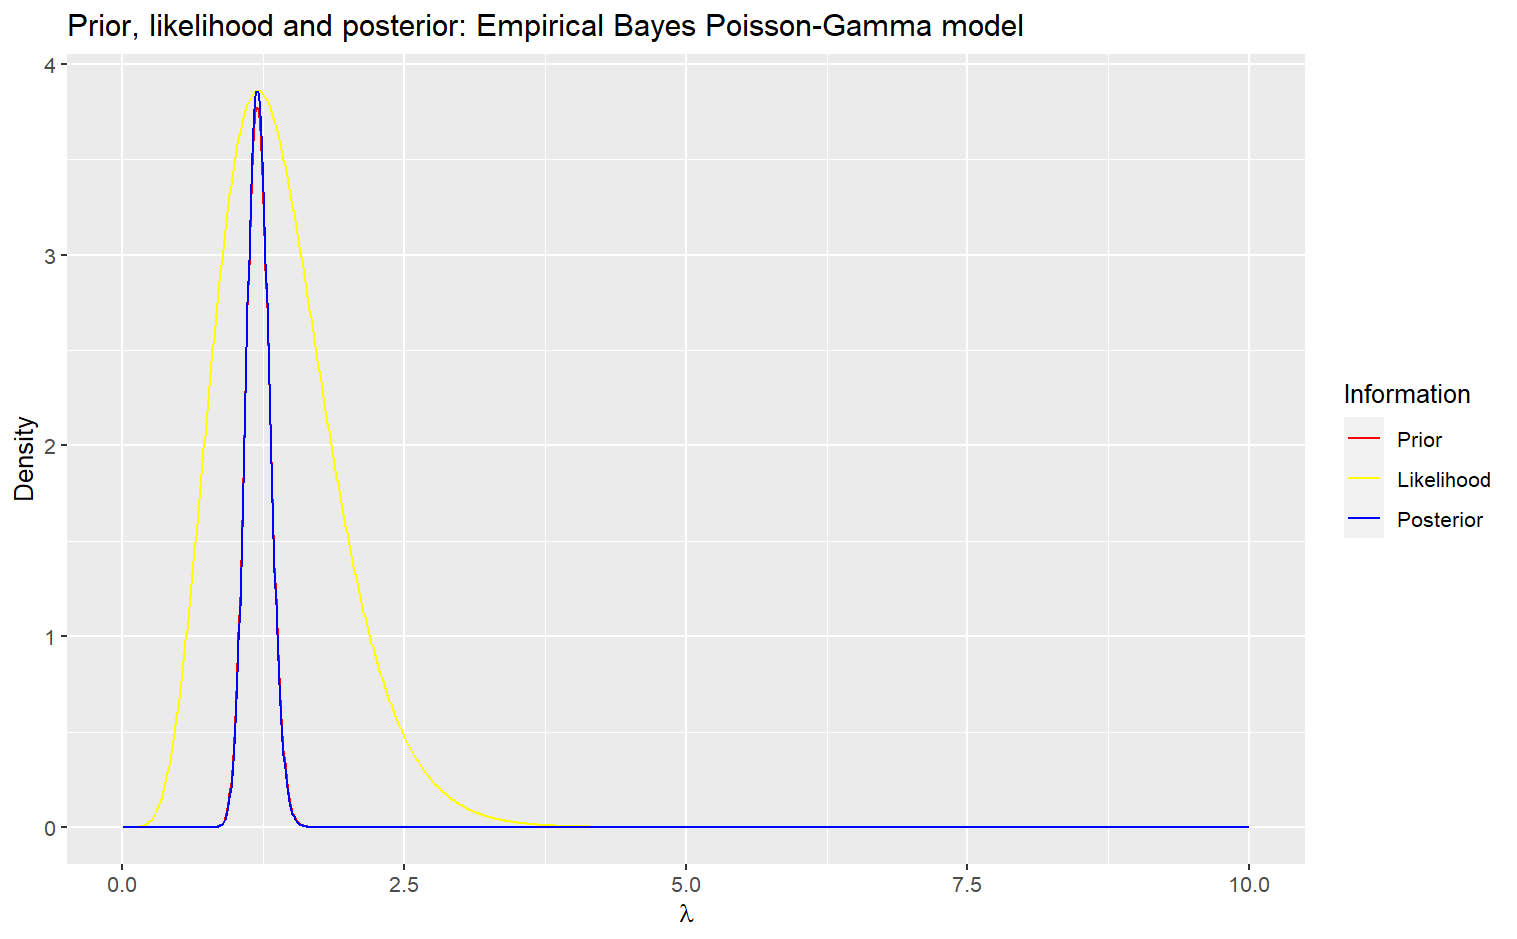
\includegraphics[width=340pt, height=200pt]{Chapters/chapter1/figures/piorlikepost.png}
	%%\centerline{\epsfig{/Chapters/chapter1/figures/cat.eps,width=.8\textheight,height=.4\textwidth}}
	\caption[List of figure caption goes here]{Prior, likelihood and posterior: Bernoulli-Beta model.}\label{fig12}
\end{figure}


\begin{tcolorbox}[enhanced,width=4.67in,center upper,
	fontupper=\large\bfseries,drop shadow southwest,sharp corners]
	\textit{R code. Car claim, predictive probabilities plots}
\begin{VF}
\begin{lstlisting}[basicstyle=\scriptsize, language=R]
# Predictive distributions
require(TailRank)

PredDen <- function(y, y0, a0, b0){
	N <- length(y)
	aN <- a0 + sum(y) # Posterior shape parameter
	bN <- b0 + N - sum(y) # Posterior scale parameter
	Pr <- aN/(aN+bN)
	Probs <- dbinom(y0, 1, prob = Pr)
	return(Probs)
}
y0 <- 0:1
PredVague <- PredDen(y = y, y0 = y0, a0 = a0, b0 = b0)
PredEB <- PredDen(y = y, y0 = y0, a0 = a0EB, b0 = b0EB)
dataPred <- as.data.frame(cbind(y0, PredVague, PredEB))
colnames(dataPred) <- c("y0", "PredictiveVague", 
"PredictiveEB")

ggplot(data = dataPred) + 
geom_point(aes(y0, PredictiveVague, color = "red")) +  
xlab(TeX("$y_0$")) + ylab("Density") +
ggtitle("Predictive density: Vague and Empirical 
Bayes priors") 
+ geom_point(aes(y0, PredictiveEB, color = "yellow")) +
guides(color = guide_legend(title="Prior")) +
scale_color_manual(labels = c("Vague", "Empirical Bayes"), 
values = c("red", "yellow")) +
scale_x_continuous(breaks=seq(0,1,by=1))

\end{lstlisting}
\end{VF}
\end{tcolorbox}

\begin{figure}[!h]
	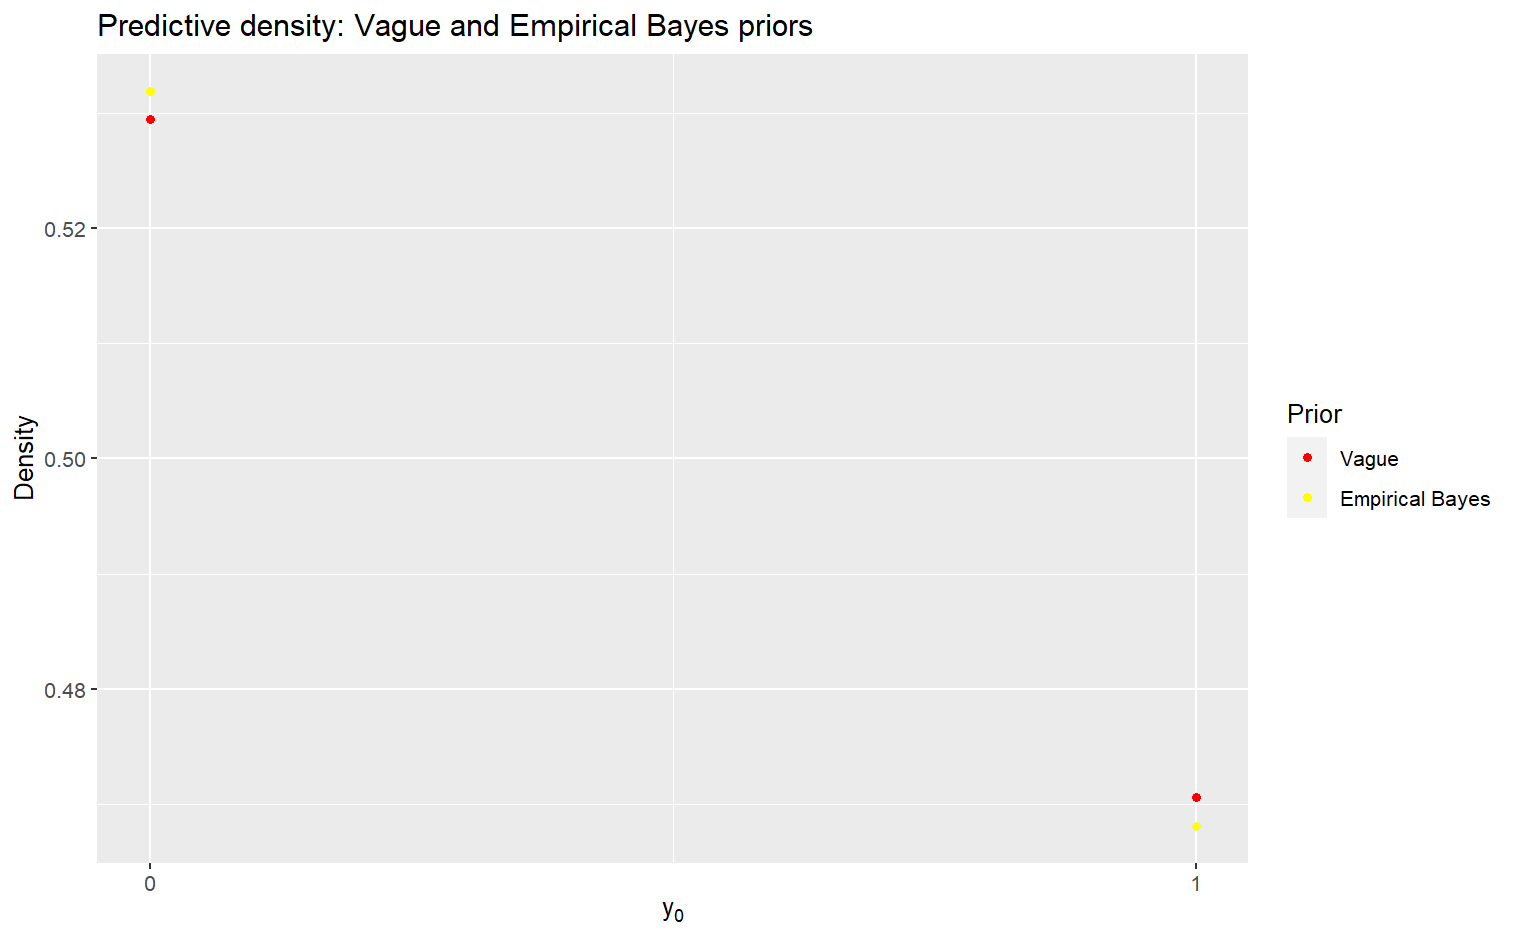
\includegraphics[width=340pt, height=200pt]{Chapters/chapter1/figures/predictive.png}
	%%\centerline{\epsfig{/Chapters/chapter1/figures/cat.eps,width=.8\textheight,height=.4\textwidth}}
	\caption[List of figure caption goes here]{Predictive probabilities: Bernoulli-Beta model.}\label{fig13}
\end{figure}

\begin{tcolorbox}[enhanced,width=4.67in,center upper,
	fontupper=\large\bfseries,drop shadow southwest,sharp corners]
	\textit{R code. Car claim, Bayesian model average}
	\begin{VF}
		\begin{lstlisting}[basicstyle=\scriptsize, language=R]
# Posterior odds: Vague vs Empirical Bayes
PO12 <- exp(-LogMgLik(c(a0EB, b0EB), y = y))/
exp(-LogMgLik(c(a0, b0), y = y))

PostProMEM <- PO12/(1 + PO12) 
# Posterior model probability Empirical Bayes
PostProMEM
0.757
PostProbMV <- 1 - PostProMEM 
# Posterior model probability vague prior
PostProbMV
0.242

# Bayesian model average (BMA)
PostMeanEB <- (a0EB + sum(y)) / (a0EB + b0EB + N) 
# Posterior mean Empirical Bayes 
PostMeanV <- (a0 + sum(y)) / (a0 + b0 + N) 
# Posterior mean vague priors
BMAmean <- PostProMEM * PostMeanEB + PostProbMV * PostMeanV  
# BMA posterior mean

PostVarEB <- (a0EB + sum(y))*(b0EB + N - sum(y)) / 
((a0EB + b0EB + N)^2)*(a0EB + b0EB + N -1) 
# Posterior variance Empirical Bayes
PostVarV <- (a0 + sum(y))*(b0 + N - sum(y)) / 
((a0 + b0 + N)^2)*(a0 + b0 + N -1) 
# Posterior variance vague prior 

BMAVar <- PostProMEM * PostVarEB + PostProbMV * PostVarV 
+ PostProMEM * (PostMeanEB - BMAmean)^2 + PostProbMV * 
(PostMeanV - BMAmean)^2
# BMA posterior variance   

# BMA: Predictive
BMAPred <- PostProMEM * PredEB + PostProbMV * PredVague    
dataPredBMA <- as.data.frame(cbind(y0, BMAPred))
colnames(dataPredBMA) <- c("y0", "PredictiveBMA")

ggplot(data = dataPredBMA) + 
geom_point(aes(y0, PredictiveBMA, color = "red")) +  
xlab(TeX("$y_0$")) + ylab("Density") +
ggtitle("Predictive density: BMA") +
guides(color = guide_legend(title="BMA")) +
scale_color_manual(labels = c("Probability"), 
values = c("red")) 
+ scale_x_continuous(breaks=seq(0,1,by=1))
			
\end{lstlisting}
\end{VF}
\end{tcolorbox}

\begin{tcolorbox}[enhanced,width=4.67in,center upper,
	fontupper=\large\bfseries,drop shadow southwest,sharp corners]
	\textit{R code. Car claim, Bayesian updating plots}
\begin{VF}
\begin{lstlisting}[basicstyle=\scriptsize, language=R]
# Bayesian updating
BayUp <- function(y, lambda, a0, b0){
 N <- length(y)
 aN <- a0 + sum(y) 
 # Posterior shape parameter
 bN <- b0 + N - sum(y)    
 # Posterior scale parameter
 p <- dbeta(lambda, shape1 = aN, shape2 = bN) 
 # Posterior density
 return(list(Post = p, a0New = aN, b0New = bN))
}
			
PostUp <- NULL
 for(i in 1:N){
 if(i == 1){
  PostUpi <- BayUp(y[i], lambda, a0 = 1, b0 = 1)}
	else{
	PostUpi <- BayUp(y[i], lambda, 
	a0 = PostUpi$a0New, b0 = PostUpi$b0New)
 }
 PostUp <- cbind(PostUp, PostUpi$Post)
}
			
 DataUp <- data.frame(cbind(rep(lambda, 15), c(PostUp),
 rep(1:15, each = 1000))) 
 #Data frame
 colnames(DataUp) <- c("Lambda", "Density", "Factor")
 DataUp$Factor <- factor(DataUp$Factor, levels=c("1","2",
 "3","4","5","6","7","8","9","10","11","12","13","14","15"), 
 labels=c("Iter_1","Iter_2","Iter_3","Iter_4","Iter_5",
 "Iter_6","Iter_7","Iter_8","Iter_9","Iter_10","Iter_11",
 "Iter_12","Iter_13","Iter_14","Iter_15"))
			
ggplot(data = DataUp, aes_string(x = "Lambda", 
 y = "Density", group = "Factor")) + 
 geom_line(aes(color = Factor)) +
 xlab(TeX("$p$")) + ylab("Density") +
 ggtitle("Bayesian updating: 
 Beta-Binomial model with vague prior") +
 guides(color=guide_legend(title="Update")) 		
\end{lstlisting}
\end{VF}
\end{tcolorbox}


\begin{figure}[!h]
	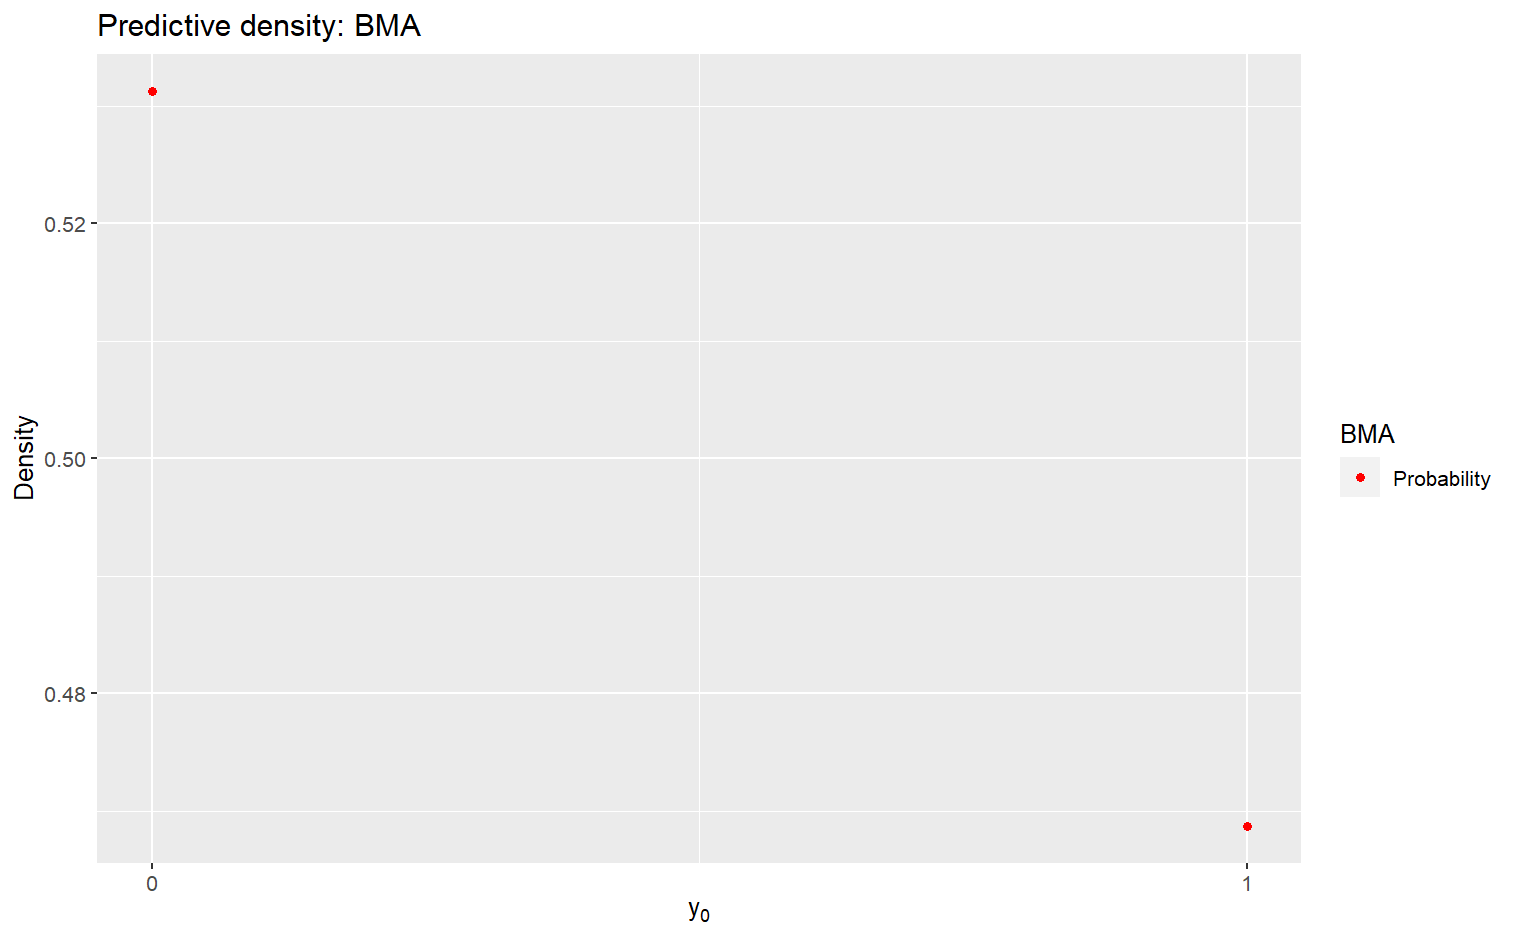
\includegraphics[width=340pt, height=200pt]{Chapters/chapter1/figures/BMA.png}
	%%\centerline{\epsfig{/Chapters/chapter1/figures/cat.eps,width=.8\textheight,height=.4\textwidth}}
	\caption[List of figure caption goes here]{Predictive probabilities: Bernoulli-Beta Bayesian model average.}\label{fig14}
\end{figure}

\begin{figure}[!h]
	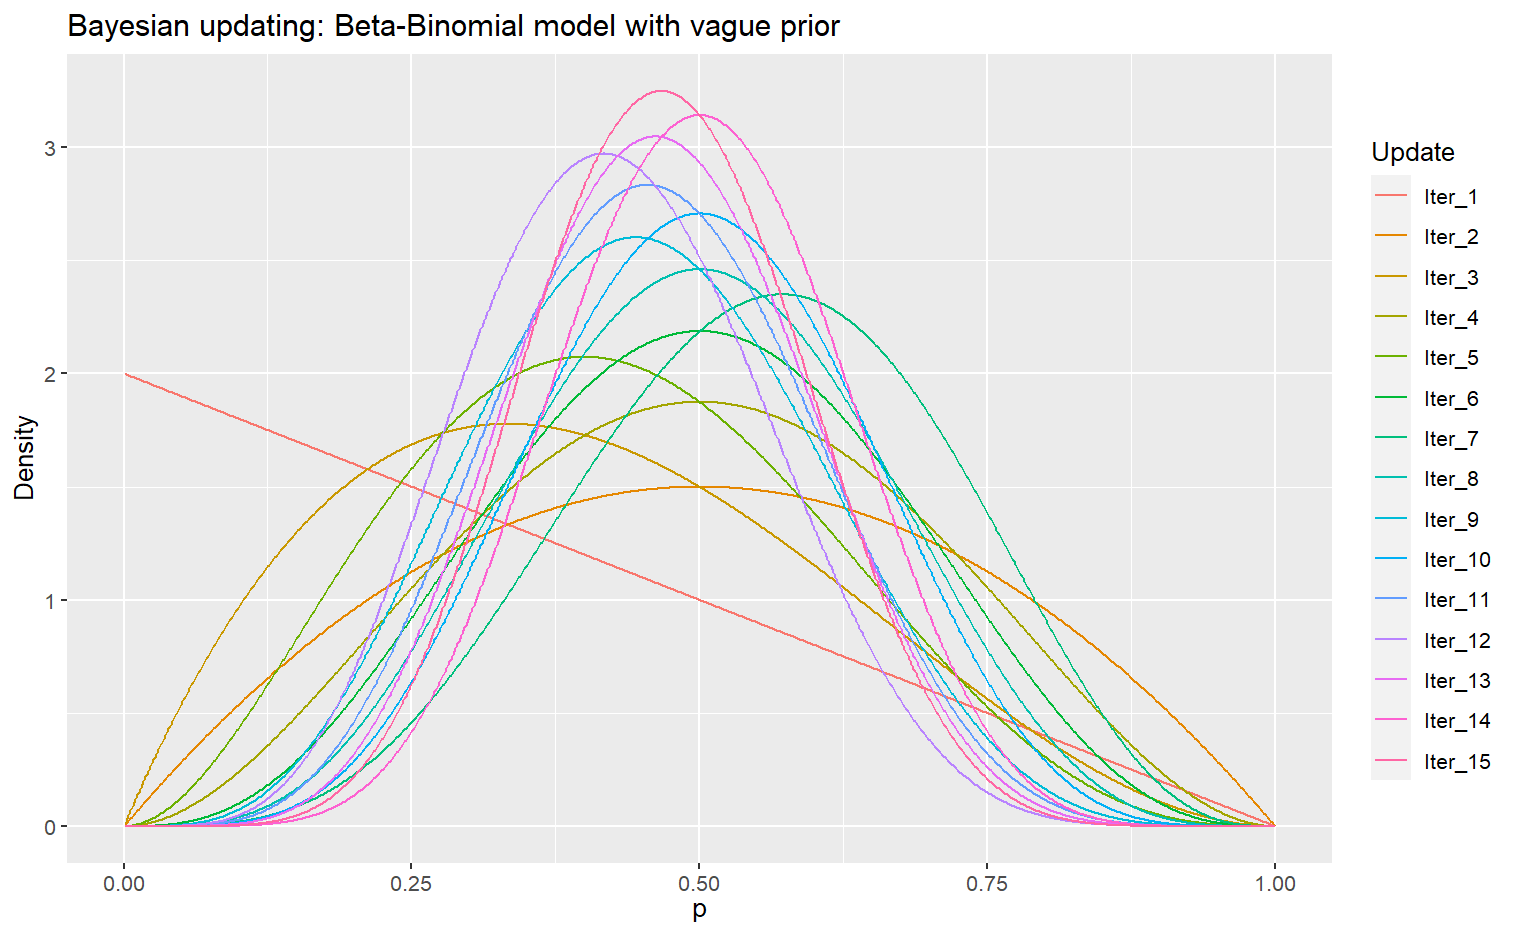
\includegraphics[width=340pt, height=200pt]{Chapters/chapter1/figures/BayesUp.png}
	%%\centerline{\epsfig{/Chapters/chapter1/figures/cat.eps,width=.8\textheight,height=.4\textwidth}}
	\caption[List of figure caption goes here]{Predictive probabilities: Bernoulli-Beta Bayesian model updating.}\label{fig15}
\end{figure}


\item Show that given the loss function, $L({\theta},a)=|{\theta}-a|$, then ${\delta}(\mathbf{y})$ is the median.

\textbf{Answer}

$\int_{{\Theta}} |{\theta}-a|\pi({\theta}|\mathbf{y})d{\theta}=\int_{-\infty}^a (a-{\theta})\pi({\theta}|\mathbf{y})d{\theta}+\int_{a}^{\infty} ({\theta}-a)\pi({\theta}|\mathbf{y})d{\theta}$. Differentiating with respect to $a$, and equating to zero,

\begin{equation}
	\int_{-\infty}^a \pi({\theta}|\mathbf{y})d{\theta}=\int_{a}^{\infty} \pi({\theta}|\mathbf{y})d{\theta},  
\end{equation}

then,

\begin{equation}
	2\int_{-\infty}^a \pi({\theta}|\mathbf{y})d{\theta}=\int_{-\infty}^{\infty} \pi({\theta}|\mathbf{y})d{\theta}=1,  
\end{equation}

that is, $a^*(\mathbf{y})$ is the median.
\end{enumerate}